\documentclass[12pt,notitlepage]{article}

\usepackage[utf8]{inputenc}
%\usepackage[english]{babel}
\usepackage[letterpaper, margin=1.4in]{geometry}
\usepackage{graphicx}
\usepackage{amsmath, amsthm, amsfonts, amssymb}
\usepackage{esint}
\usepackage{url}
\usepackage{verbatim}
\usepackage{hyperref}
\usepackage{siunitx}
\usepackage{array}
\usepackage{tabu}
\usepackage{gensymb}
\usepackage{grffile}
\usepackage{float}
\usepackage{algorithm}
%\usepackage{algorithmic}
\usepackage{algorithmicx}
\usepackage{algpseudocode}

\usepackage{fancyhdr}
\pagestyle{fancy}
\fancyhf{}
\fancyhead[L]{\emph{L. Karlsson; version 0.4}}
\fancyhead[R]{\emph{\leftmark}}
\fancyfoot[C]{\thepage}

\newtheorem{theorem}{Theorem}

\title{Thesis Project Plan\\SF250X}
\author{Ludwig Karlsson\\ludwigka@kth.se}
\date{2023-01-12}

\begin{document}
\maketitle

\section{Background}
A MultiProcessor System on Chip (MPSoC) is a system of multiple microprocessors integrated on a single chip. The microprocessors are often heterogeneous and can include for example Central Processing Units (CPUs), Graphics Processing Units (GPUs), and Field Programmable Gate Arrays (FPGAs) depending on the target application of the chip. FPGAs are integrated circuits that provide a configurable and highly parallel computational resource. FPGAs are widely used for applications where production size is too low to motivate custom Application-Specific Integrated Circuits (ASICs), for prototyping to reduce iteration cost, as hardware accelerators where their ability to process a lot of data in parallel can be used, and for applications where the ''hardware'' needs to be reconfigured frequently.

When designing or choosing a system (for example an MPSoC) for a particular application, it is often desirable to pick the ''cheapest'' allowable hardware configuration for the task (according to some metric, for example power consumption or hardware cost). It is also often desirable to schedule/map different processes to hardware resources as efficiently as possible, for example to maximize data throughput, or to be able to use less resources to reduce power consumption or leave the resources available for other tasks\footnote{E.g. given some hardware it is desirable to use it as efficiently as possible, and given some task it is desirable to use as little computational resources as possible to run it.}. The process of finding optimal configurations is known as Design Space Exploration (DSE). In general, the DSE task is NP-complete and has historically been a largely manual process. More or less automated ways of doing DSE has been developed where the goal is to use optimization techniques to find good solutions within a space of design criteria that satisfy some system requirements and often maximize/minimize some cost metrics. These methods often utilize heuristics or manual input to reduce the problem size. Heterogeneous MPSoCs with FPGAs provide a particularly difficult situation where the properties of the different hardware resources and the reconfigurability of the FPGAs make the design space very large. Design Space Identification (DSI) is a systematic approach to converting simpler models of hardware and a computational problem to a combined form that can be used within DSE [1].

\section{Application}
This project is concerned with an application at Saab of DSE on a Xilinx MPSoC with CPU, GPU, and reconfigurable FPGA resources. The use case concerns a dynamic scenario where different processes with different priorities need to be scheduled and run on the chip. The processes can run on some combination of the chip's resources (eg. a certain process may be able to run on a CPU core or on the FPGA), and the ultimate goal is to determine a way to schedule processes on the available resources including possible reconfigurations of the FPGA that results in performance that is as close to optimal as possible.

\subsection{Mathematical/Numerical Aspects}
Finding the optimal solution to the design-space problem is an NP-complete problem. Historically, computational DSE has been limited by computational resources, and approaches have required limiting assumptions or have been largely heuristical. These methods tend to give solutions that are good but not optimal, and they can sometimes be improved considerably. Kathrin Rosvall and Rodolfo Jordão have as part of Ingo Sander's research group showcased an approach that based on a discrete model of the system and computational problem utilizes Constraint Programming (CP) and a combination of heuristics and search that limits the design space without removing any feasible solutions. This makes it possible to obtain a feasible solution fairly quickly, and then eventually prove optimality if the problem is small enough [2]. This project aims to build on these methods by extending the IDeSyDe tool [3] within the ForSyDe framework [4]. The key focus will be to investigate Saab's problem with the current CP approach as well as with some other solver in order to see what method works best for this problem.

The full scope of adapting the IDeSyDe tool to Saab's application, and answering all of Saab's questions in the general dynamic load case scenario is an extremely complex problem and outside of the reasonable scope of this project. In order to obtain a more reasonable problem formulation, this project will instead restrict the problem formulation to some static load case scenario and aim to adapt the current tool-set to the problem when possible. Numerical aspects of the method will be investigated in particular, and how numerical considerations compare between the methods.
\newline\newline
\noindent\textbf{Research question}:

To what extent can the IDeSyDe tool and different optimisation methods be used to answer Saab's questions regarding task mapping and scheduling? Is the abstraction level of IDeSyDe appropriate to the problem and what parts of the system are best suited for this approach? What tools are most appropriate for the problem or different part of the problem: how do they compare and what numerical considerations are relevant?

\section{Initial Plan}
The goals for the project is to:
\begin{enumerate}
	\item[G1] Find an interesting static load case scenario. Research and formulate good models for Saab's hardware and application. Figure out how to measure/quantify the performance boost. Research relevant numerical aspects.
	\item[G2] Extend IDeSyDe with models and meta-heuristics.
	\item[G3] Investigate Saab's questions within the limitations of the static load case scenario and the model.
	\begin{enumerate}
		\item Look at the current CP approach and some other approach.
		\item Investigate trade-offs between performance (of the solution) and computational cost for different solvers and heuristics, as well as numerical considerations.
		\item Look at ways to extend/modify the model to reduce computational cost and/or improve performance.
	\end{enumerate}
\end{enumerate}

\noindent Figure \ref{timeplan} shows a preliminary time plan for the project. The report will be worked on in parallel with the other project work for the duration of the project.

\begin{figure}[H]
	\centering
	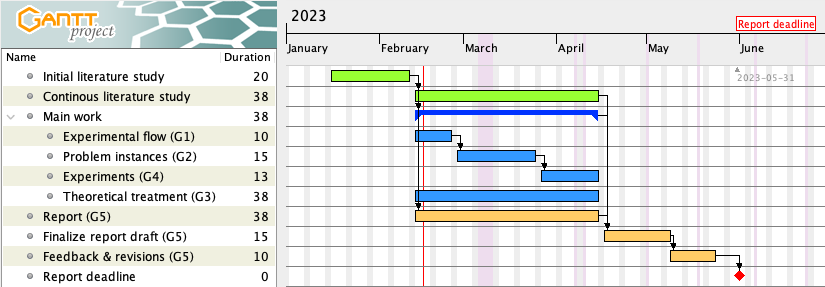
\includegraphics[scale=0.5]{figures/timeline.png} 
	\caption{Preliminary time plan for the project.}
	\label{timeplan}
\end{figure}

%\begin{table}[H]
%	\centering
%	\begin{tabular}{c|l}
%		Week(s) & Task \\
%		\hline
%		3-5 & Literature study. \\
%		6-8 & Application \& platform model. [S1-S2] \\
%		9-14 & S3 \\
%		15-17 & Evaluation on hardware. [S4] \\
%		18-20 & Report draft. \\
%		21 & Revisions and final report deadline.
%	\end{tabular}
%    \caption{Preliminary time plan for the project.}
%	\label{timeplan}
%\end{table}

\section{References}
\begin{enumerate}
\item R. Jordão, I. Sander and M. Becker, "Formulation of Design Space Exploration Problems by Composable Design Space Identification," 2021 Design, Automation \& Test in Europe Conference \& Exhibition (DATE), 2021, pp. 1204-1207, doi: 10.23919/DATE51398.2021.9474082.
\item Kathrin Rosvall and Ingo Sander. 2017. Flexible and Tradeoff-Aware Constraint-Based Design Space Exploration for Streaming Applications on Heterogeneous Platforms. ACM Trans. Des. Autom. Electron. Syst. 23, 2, Article 21 (March 2018), 26 pages. \url{https://doi.org/10.1145/3133210}
\item IDeSyDe repository and documentation: \url{https://github.com/forsyde/IDeSyDe/}
\item ForSyDe website: \url{https://forsyde.github.io/}
\end{enumerate}

\end{document}